\documentclass[a4paper]{article}
\usepackage[utf8]{inputenc}
\usepackage{graphicx}
\usepackage{epstopdf}
\usepackage{epsfig}
\usepackage{wrapfig}
\usepackage{subcaption}
\usepackage{float}
\usepackage{listings}
\usepackage{mathtools}
\usepackage[english,serbian]{babel}
\usepackage[usenames,dvipsnames]{color}

% This is the color used for MATLAB comments below
\definecolor{MyDarkGreen}{rgb}{0.0,0.4,0.0}

% For faster processing, load Matlab syntax for listings
\lstloadlanguages{Matlab}%
\lstset{language=Matlab,                        % Use MATLAB
        frame=single,                           % Single frame around code
        basicstyle=\small\ttfamily,             % Use small true type font
        keywordstyle=[1]\color{Blue}\bfseries,        % MATLAB functions bold and blue
        keywordstyle=[2]\color{Purple},         % MATLAB function arguments purple
        keywordstyle=[3]\color{Blue}\underbar,  % User functions underlined and blue
        identifierstyle=,                       % Nothing special about identifiers
                                                % Comments small dark green courier
        commentstyle=\usefont{T1}{pcr}{m}{sl}\color{MyDarkGreen}\small,
        stringstyle=\color{Purple},             % Strings are purple
        showstringspaces=false,                 % Don't put marks in string spaces
        tabsize=5,                              % 5 spaces per tab
        %
        %%% Put standard MATLAB functions not included in the default
        %%% language here
        morekeywords={xlim,ylim,var,alpha,factorial,poissrnd,normpdf,normcdf},
        %
        %%% Put MATLAB function parameters here
        morekeywords=[2]{on, off, interp},
        %
        %%% Put user defined functions here
        morekeywords=[3]{FindESS, homework_example},
        %
        morecomment=[l][\color{Blue}]{...},     % Line continuation (...) like blue comment
        numbers=left,                           % Line numbers on left
        firstnumber=1,                          % Line numbers start with line 1
        numberstyle=\tiny\color{Blue},          % Line numbers are blue
        stepnumber=5                            % Line numbers go in steps of 5
}

\begin{document}

\title{Logistička modifikacija Lotka-Voltera modela\\
	\small{Seminarski u okviru kursa\\Osnove matematičkog modeliranja\\Matematički fakultet}
}
\author{Marina Brkić, Nikola Vlahović\\marinabrkic91@gmail.com\\nikola.vlahovic2401@gmail.com}
\date{27. ~maj 2018.}
\maketitle
\abstract{
	Lotka-Voltera nelinearne diferencijalne jednačine prvog reda
	se koriste za modeliranje bioloških, hemijskih i ekonomskih sistema.
	Kroz primer interakcije lisica i zečeva, predstavljamo standardne jednačine i
	modifikaciju koja uzima u obzir ograničen kapacitet staništa.

	Ključne reči: Lotka-Voltera jednačine, modeliranje populacija, predator-plen
}
\tableofcontents

\newpage

\section{Uvod}
\label{sec:uvod}

Alfred J. Lotka je u svom radu ``Doprinos teoriji periodičnih reakcija'' objavljenom 1910. godine predstavio
inicijalnu formulaciju Lotka-Voltera jednačina za modeliranje ponašanja određenih hemijskih reakcija, koju
1920. koristi za modeliranje sistema u kom interaguju biljka i biljojed. Pet godina kasnije objavljuje knjgu
gde pomoću ovih jednačina modelira populacije plena i grabljivice. Te jednačina objavljuje i Vito Voltera
u radu gde analizira populacije riba u Jadranskom moru, nakon što je kroz razgovor sa svojim budućim zetom,
morskim biologom Umbertom D'Ankonom, saznao da je nakon rata porastao procenat ulovljenih grabljivih riba.
\\\\
Ilustrovaćemo kroz primer lisica i zečeva primenu Lotka-Voltera jednačina na modeliranje
populacija sa plen-grabljivica interakcijama.

\section{Standardni Lotka-Voltera model}
\label{sec:std_model}
Stanište dele populacije lisica i zečeva. Lisice se hrane isključivo zečevima,
dok za zečeve uvek ima hrane u izobilju. Populacija zečeva bi u nedostatku lisica
neprestano rasla. Obratno, populacija lisica bi u slučaju nedostatka zečeva (hrane) ubrzo izumrla.
Označimo broj zečeva sa x(t), a broj lisica sa y(t) za vreme t.
Jednačine:
    \begin{equation}
        \begin{aligned}
	    x' = ax \\
        y' = -my
        \end{aligned}
	\end{equation}
gde su a i m parametri koji predstavljaju stope rasta i odumiranja odgovarajućih populacija,
ilustruju njihovo ponašanje u nedostatku interakcije.
Da bismo dobili realističniji model, neophodno je da inkorporiramo u jednačine
činjenicu da lisice love zečeve. Broj njihovih susreta je direktno proporcionalan
brojnosti lisica i zečeva, što možemo modelirati proizvodom xy. Lov izaziva opadanje
populacije zečeva, dok omogućava porast populacije lisica.
Neka su b i c koeficijenti smrtnosti zečeva tj.
nataliteta lisica pri omogućenim interakcijama, i pretpostavimo da su lisice uvek gladne,
tj. da će svakom ukazanom prilikom pojesti zeca.
Promene populacija možemo modelirati \textbf{Lotka-Voltera sistemom diferencijalnih jednačina}:
        \begin{equation}
        \label{eq:standard_lv}
            \begin{aligned}
                x' = ax - bxy,   x(0)=x_0\\
                y' = -my + cxy,  y(0)=y_0
            \end{aligned}
		\end{equation}

Iz jednačina sledi da će porast populacije zečeva kao posledicu omogućiti porast populacije lisica,
ali kako populacija lisica raste, usled povećanog lova populacija zečeva će opadati.
Dalje, kako se bude smanjivala količina hrane za lisice, tako će i njihov broj morati da opadne.

\subsection{Stacionarna rešenja sistema}

Stacionarno rešenje definišemo kao stanje u kom ne dolazi do promena vrednosti, tj.
gde važi $x' = 0$ i $y' = 0$.
Transformišući jednačine \eqref{eq:standard_lv} dobijamo
    \begin{displaymath}
        \begin{aligned}
            x' = x (a - by) = 0\\
            y' = y (cx - m) = 0
        \end{aligned}
    \end{displaymath}

gde za netrivijalna rešenja važi
    \begin{displaymath}
        \begin{aligned}
            a - by = 0\\
            cx - m = 0
        \end{aligned}
    \end{displaymath}

iz čega jednostavnim transformacijama dobijamo
    \begin{equation}
        \label{eq:stac_sol_std}
        \begin{aligned}
            x = \frac{m}{c} \equiv x_s\\
            y = \frac{a}{b} \equiv y_s.
        \end{aligned}
    \end{equation}

\subsection{Analitičko rešenja sistema}

Sistem \eqref{eq:standard_lv} se može pomoću \eqref{eq:stac_sol_std}
napisati u obliku
\begin{displaymath}
    \begin{aligned}
        x' = ax(1 - \frac{by}{a}) = ax(1 - \frac{y}{y_s})\\
        y' = -my(1 - \frac{cx}{m}) = -my(1 - \frac{x}{x_s}).
    \end{aligned}
\end{displaymath}

Uvodimo smene $z(t) = \frac{x(t)}{x_s}$ i $l(t) = \frac{y(t)}{y_s}$

\begin{displaymath}
    \begin{aligned}
        z' = al(1 - l)\\
        l' = -mz(1 - z)
    \end{aligned}
\end{displaymath}

iz čega se može dobiti
\begin{displaymath}
    \begin{aligned}
        al(1 - l) \frac{dz}{dl} = -mz(1 - z).
    \end{aligned}
\end{displaymath}

Ako podelimo ovu jednačinu sa $xz$, dobijamo
\begin{displaymath}
    \begin{aligned}
        a(z - 1) \frac{dz}{dl} = -m(l - 1).
    \end{aligned}
\end{displaymath}

Integralimo obe strane po $dl$
\begin{displaymath}
    \begin{aligned}
        \int a(z - 1) \frac{dz}{dl} dl= \int -m(l - 1) dl
    \end{aligned}
\end{displaymath}

i dobijamo jednačinu

\begin{displaymath}
    \begin{aligned}
        a(\ln z -z) + C_1 = -m(\ln l - l) + C_2\\
        a(\ln z -z) + m(\ln l - l) = C
    \end{aligned}
\end{displaymath}

\subsection{Primer u Matlabu}
\label{sub:std_primer}
Da bi rešili ovaj sistem jednačina koristićemo Matlab funkciju ode45. Ova funkcija koristi Runge-Kuta
formule četvrtog i petog stepena za automatsko integrisanje.\\ \\
Naše jednačine su
    \begin{equation}
        \begin{aligned}
            x' = ax - bxy \\
            y' = -yc + mxy
        \end{aligned}
	\end{equation}
Kada ubacimo vrednosti parametara koje su $a=3, b=2, c=1, m=2.5$ i jednačine izjednačimo sa 0, dobijamo:
    \begin{equation}
        \begin{aligned}
            x'=3x - 2xy = 0 \\
            y'=-y + 2.5xy = 0
        \end{aligned}
	\end{equation}
U Matlabu pravimo m fajl $ standard\_equations.m $:

\lstinputlisting{../standard_equations.m}

\begin{figure}[H]
    \centering
    \begin{minipage}{0.45\textwidth}
        \centering
        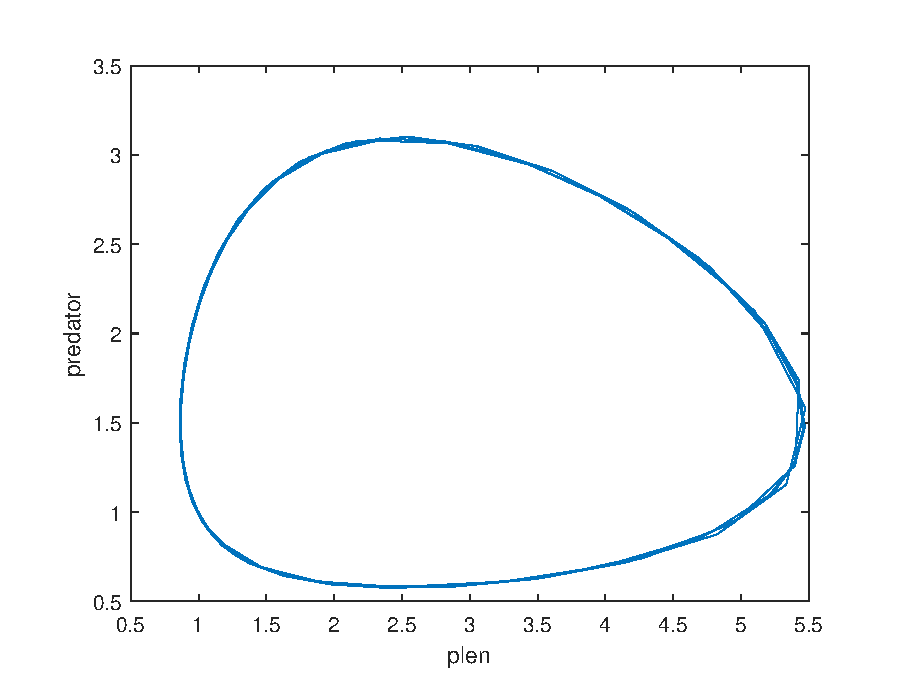
\includegraphics[width=1\textwidth]{images/lotka_voltera_phase} % first figure itself
        \caption{Fazni dijagram standardnog modela}
    \end{minipage}\hfill
    \begin{minipage}{0.45\textwidth}
        \centering
        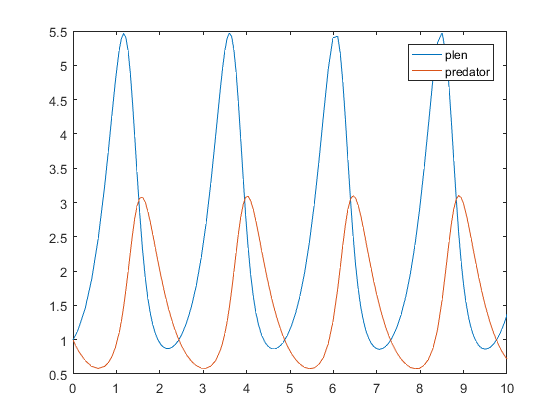
\includegraphics[width=1\textwidth]{images/lotka_voltera_time_plot} % second figure itself
        \caption{Grafik promene populacija kroz vreme za standardni model}
    \end{minipage}
\end{figure}

\section{Logistička modifikacija Lotka-Voltera modela}
\label{sec:log_mod}
Može se videti da je prethodni model realističan dokle god je koeficijent priraštaja zečeva konstantan.\\
Znamo da na realnom, konačnom staništu populacija ne može neograničeno rasti zbog
ograničenih raspoloživih resursa. Dakle, stanište može da podrži odredjen maksimalan broj
jedinki neke vrste. Označimo taj broj sa $U$. Iskoristivši pretpostavku
da priraštaj linearno zavisi od veličine populacija, belgijski matemaričar Verhulst je predložio model:
	\begin{equation}
		\frac{dN(t)}{dt}=rN (t) (1 - \frac{N (t)}{U})
	\end{equation}
Ako primenimo logističku formulu u računanju priraštaja populacije zečeva, uračunavamo i zavisnost
od odnosa veličine populacije i kapaciteta staništa.\\
Time se dobijaju jednačine:

    \begin{equation}
        \begin{aligned}
            x' = ax(1 - \frac{x}{U}) - bxy\\
            y' = -my + cxy
        \end{aligned}
	\end{equation}

\subsection{Primer u Matlabu}
\label{sub:log_mod_matlab}

\lstinputlisting{../logistic_equations.m}

\begin{figure}[H]
    \centering
    \begin{minipage}{0.45\textwidth}
        \centering
        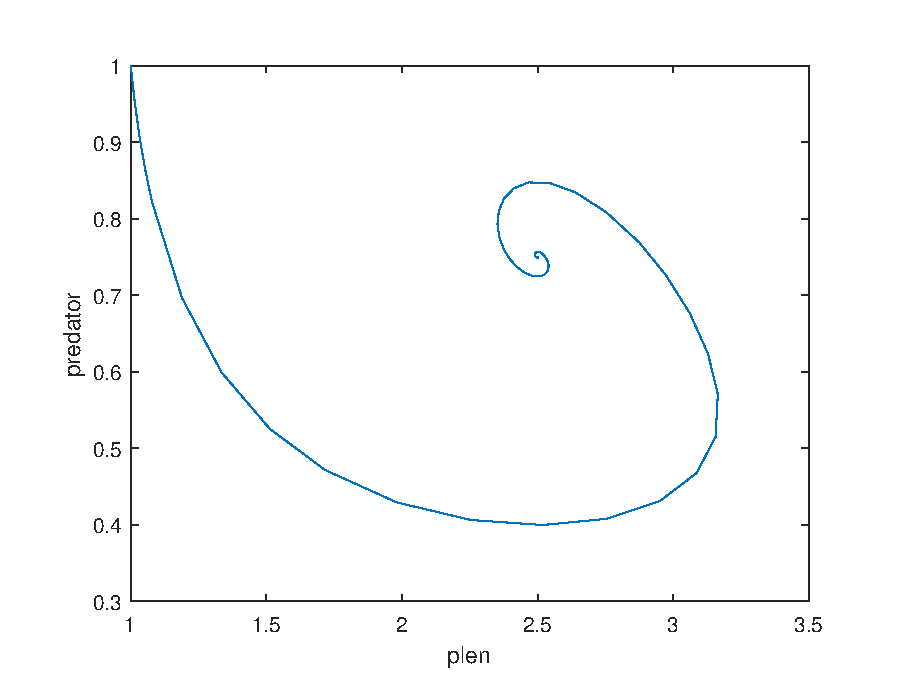
\includegraphics[width=1\textwidth]{images/lotka_voltera_logistic_phase} % first figure itself
        \caption{Fazni dijagram za U=5}
    \end{minipage}\hfill
    \begin{minipage}{0.45\textwidth}
        \centering
        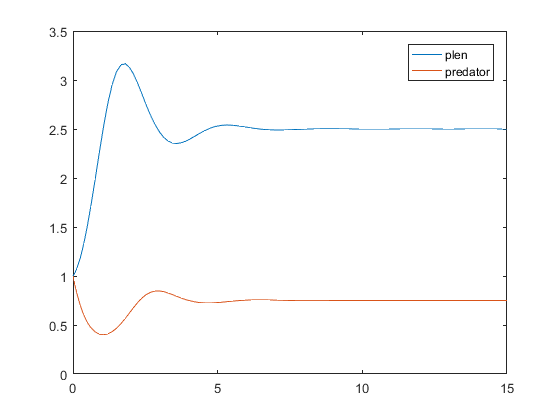
\includegraphics[width=1\textwidth]{images/lotka_voltera_logistic_time_plot} % second figure itself
        \caption{Promena populacija za U=5}
    \end{minipage}
\end{figure}

\subsection{Statičko rešenje za model sa logističkom modifikacijom}

\subsection{Stanište sa vrlo ograničenim kapacitetom}
\label{sub:log_mod_ogr}

Koristimo isti model sa parametrima $a=3, b=2, c=1, m=2.5, U=2$
i početnom konfiguracijom $x(0)=1, y(0)=1$.
Sa grafikona vidimo da populacija plena ne raste dovoljno brzo da omogući
održanje lisica na staništu.

\begin{figure}[H]
    \centering
    \begin{minipage}{0.45\textwidth}
        \centering
        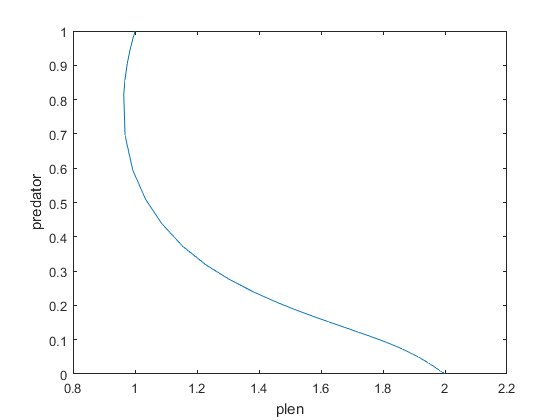
\includegraphics[width=1\textwidth]{images/lv_low_u_phase} % first figure itself
        \caption{Fazni dijagram za U=2}
    \end{minipage}\hfill
    \begin{minipage}{0.45\textwidth}
        \centering
        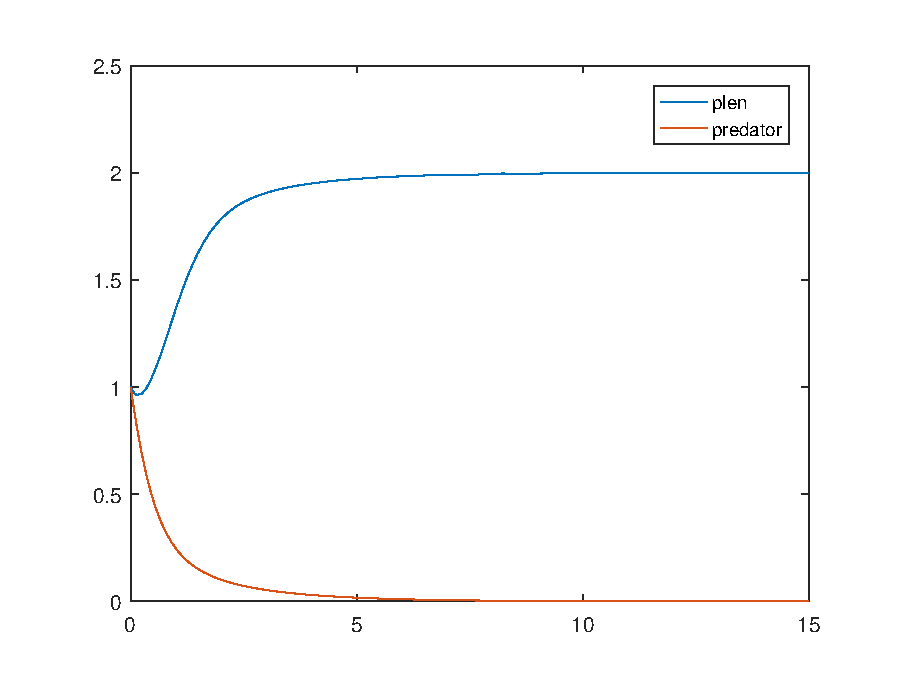
\includegraphics[width=1\textwidth]{images/lv_low_u_time} % second figure itself
        \caption{Promena populacija za U=2}
    \end{minipage}
\end{figure}

\section{Zaključak}
\label{sec:zakljucak}

Osnovni Lotka-Voltera model je dobar za modeliranje vrlo jednostavnih sistema,
ali kod kompleksnijih sistema, sa više interakcija i kompleksnijim parametrima ne uspeva
da realistično predstavi situaciju. Sa druge strane, usled svoje elegancije i jednostavnosti,
izuzetno ga je lako modifikovati ili inkorporirati u druge modele, što ga čini relevantnim i danas.

\end{document}